\chapter{Materiales y metodos} % Main chapter title

\label{Chapter2}

%----------------------------------------------------------------------------------------
%	SECTION 1
% Aquí se mencionan los componentes que se utilizaron y la metodología empleada.
% Luego pueden ir las plaquetas que se diseñaron para el prototipo, esquemáticos,
% diagrama de flujo, dibujos en 3D, etc.
%----------------------------------------------------------------------------------------

\section{Dispositivos y herramientas utilizadas}

Para la implementación del presente trabajo se utilizó:
\begin{itemize}
\item Placa ADC-SoC de TerasIC.
\item Software Quartus Prime.
\item Software ModelSim.
\item Extractor analógico.
\item Simulador de radar.

\end{itemize}

\subsection{Placa ADC-SoC de TerasIC}
Es una placa tipo SoC-FPGA. El circuito de conversión analógica a digital incorporado utiliza conectores SMA como interfaz de entrada y proporciona dos canales de conversión, cada uno de 14-bits de resolución y una frecuencia de muestreo de hasta 150 MSPS (Megasamples per Second).

\begin{figure}
\centering
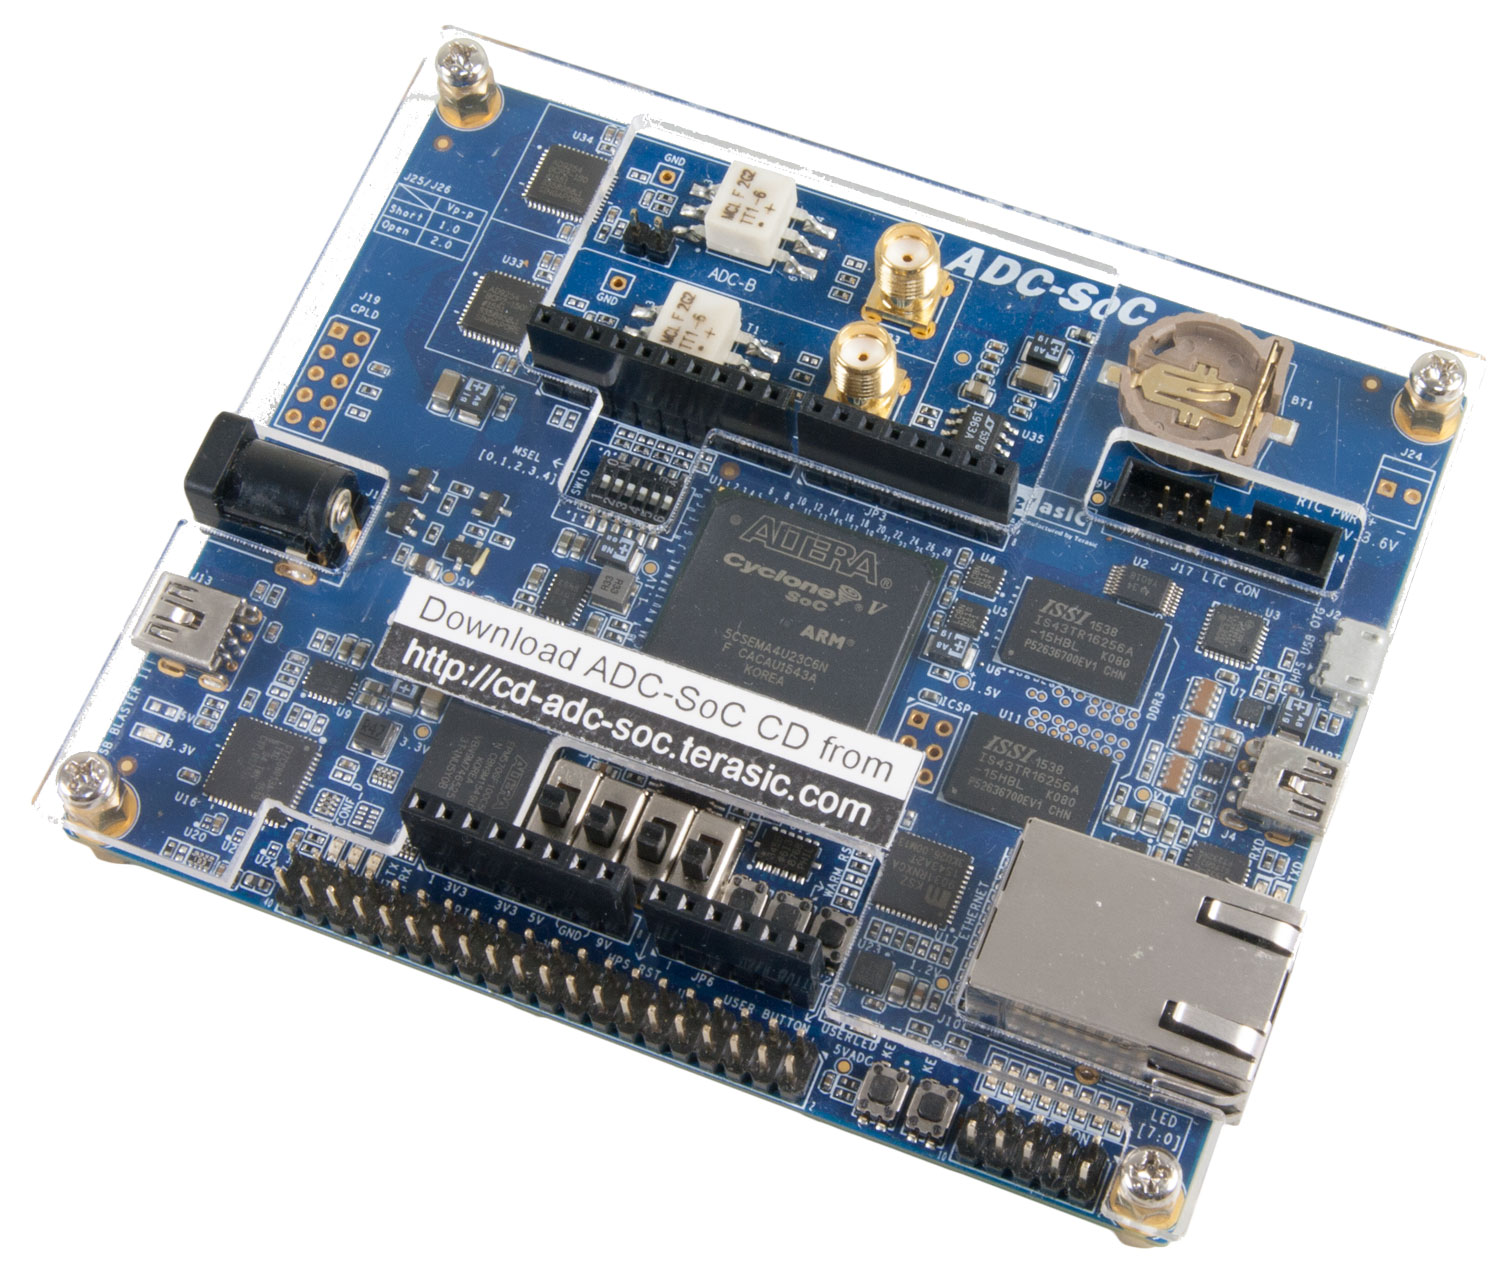
\includegraphics[scale=0.15]{./Figures/ADC-SoC.jpg}
\caption{Placa ADC-SoC de TerasIC}
\end{figure}

El siguiente hardware se proporciona en la placa:

\begin{itemize}
\item 	FPGA
	\begin{itemize}
	\item Dispositivo Altera Cyclone® V.
	\item Dispositivo de configuración en serie.
	\item USB-Blaster II integrado para programación; Modo JTAG
	\item 2 pulsadores
	\item 4 interruptores deslizantes
	\item 8 LED de usuario verdes
	\item Tres fuentes de reloj de 50 MHz del generador de reloj
	\item Un cabezal de expansión de 40 pines
	\item Un encabezado de expansión Arduino (compatibilidad con Arduino Uno R3) donde se 					puede conectar con los 'shields' Arduino.
	\item Un encabezado de expansión de entrada analógica de 10 pines (compartido con la 				entrada analógica Arduino).
	\item Convertidor A / D, interfaz SPI de 4 pines con FPGA
	\item  Dos convertidores AD de 14 bits con 150 MSPS (megamuestras por segundo)
	\end{itemize}
\item HPS (Hard Processor System)
	\begin{itemize}
	\item Procesador ARM Cortex-A9 de doble núcleo de 925 MHz
	\item 1GB DDR3 SDRAM (bus de datos de 32 bits)
	\item 1 Gigabit Ethernet PHY con conector RJ45
	\item Puerto USB OTG, conector USB Micro-AB
	\item Toma de tarjeta micro SD
	\item Acelerómetro (interfaz I2C + interrupción)
	\item UART a USB, conector USB Mini-B
	\item Botón de reinicio en caliente y botón de reinicio en frío
	\item Un botón de usuario y un LED de usuario
	\item Cabecera de expansión LTC 2x7
	\item RTC integrado (reloj en tiempo real)
	\end{itemize}
\end{itemize}


\begin{figure}
\centering
\includegraphics[scale=0.25]{./Figures/ADC-SoC_blockdiagram.jpg}
\caption{Diagrama en bloques de la placa ADC-SoC de TerasIC}
\end{figure}


En el chip Cyclone V de Altera (propiedad de Intel) se integra una FPGA y un HPS unidos por un puente HPS. Por defecto, la tarjeta micro SD tiene instalado el SO “​Linux Yocto Poky 8.0​”, el cual permite correr programas compilados en lenguaje C/C++ entre otros.
 
 
\subsection{Quartus Prime}
Quartus Prime es una herramienta de software producida por Altera para el análisis y la síntesis de diseños realizados en HDL. Permite compilar diseños, realizar análisis temporales, examinar diagramas RTL y configurar el dispositivo de destino con el programador.

Proporciona herramientas para trabajar en diferentes fases del diseño en FPGA como la creación del diseño, el agregado de restricciones, la compilación, el análisis de tiempos y la configuración de la FPGA con un promagrador. Se describen las características de Quartus a continuación:

\begin{itemize}
\item
Creación del diseño: Es posible diseñar en nivel RTL con lenguajes VHDL, Verilog o SystemVerilog. Además posee una herramienta llamada Platform Designer que crea automáticamente la lógica de interconexión a partir de la conectividad de alto nivel que se especifique. La automatización de interconexión elimina la laboriosa tarea de especificar conexiones HDL a nivel del sistema. De esta manera se pueden  especificar los requisitos de la interfaz e integrar componentes de IP dentro de una representación gráfica del sistema. En el presente proyectó se utilizó Platform Designer para configurar el puente HPS.
\item
Permite el agregado de restricciones al diseño con herramientas denominadas assigment editor y pin planner.
\item
Permite compilar el diseño, compuesto por las siguientes etapas:
\begin{itemize}
	\item
	Análisis y Síntesis
	Se evalúa el código para detectar la correcta escritura del mismo y se verifica que el mismo sea sintetizable, es decir que pueda ser implementado con lógica.
	\item
	Fitter (Colocación y Ruteo, Place \& Route): Se asignan recursos específicos de la FPGA para cumplir con el diseño. En etapa etapa además la herramienta utiliza la información sobre las restricciones de tiempo evaluar qué celdas utilizar (en terminos de distancia). Por otro lado, luego de la colocación, se emplean técnicas de optimización en la asignación de recursos.
	\item
	Generación de archivos de programación: Se generan los archivos necesarios para programar la FPGA.
	\item
	Análisis de tiempos: Se verifica que se cumplan con las restricciones de tiempo especificadas en el diseño. Por ejemplo los referidos a la generación de señales de reloj internas, derivadas de fuentes de señales de reloj externas.
	\end{itemize}
	
\item 
Posee una herramienta llamada Signal Tab Logic Analyzer que permite realizar un debug mientras el sistema se ejecuta en la FPGA.

\end{itemize}

\subsubsection{Visores de netlist}
A medida que los diseños de FPGA crecen en tamaño y complejidad, la capacidad de analizar, depurar, optimizar y restringir el diseño es fundamental. Quartus posee visores llamados RTL Viewer, State Machine Viewer y Technology Map Viewer. Cada uno permite ver representaciones esquemáticas de la estructura interna del diseño. Cada visor muestra una vista única del netlist (lista de redes) que se producen en diferentes etapas de la compilación, como se ilustra en la figura \ref{fig:netlist_viewers}. Se describen a continuación:

\begin{figure}
\centering
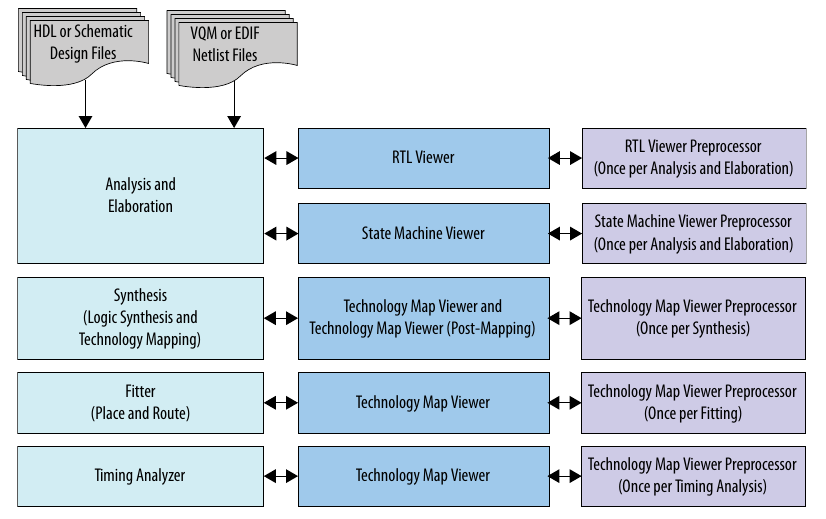
\includegraphics[scale=0.5]{./Figures/netlist_viewers.png}
\caption{Ubicación de los visores de netlist en el flujo de diseño de Quartus}
\label{fig:netlist_viewers}
\end{figure}

\begin{itemize}
\item
RTL Viewer:
Permite ver un esquema de la lista de conexiones de diseño después de la etapa de Análisis y elaboración y de la extracción de la lista de conexiones, pero antes de la síntesis y las optimizaciones de ajuste. Esta vista no es la estructura final del diseño, porque no se incluyen todas las optimizaciones; en cambio, es la vista más cercana posible al diseño original. Si el diseño utiliza síntesis integrada, esta vista muestra cómo el Quartus interpreta los archivos de diseño; Si está utilizando una herramienta de síntesis de EDA de terceros, esta vista muestra la lista de conexiones escrita por la herramienta de síntesis de EDA.

\item
State Machine Viewer
Proporciona una vista de alto nivel de las máquinas de estados finitos en el diseño y muestra la estructura interna de las máquinas de estados en el diseño, incluida una vista más detallada de la entrada y salida de los nodos de estado individuales. También muestra las transiciones de los nodos en formato de tabla.

\item
Technology Map Viewer
Permite ver un esquema de bajo nivel específico de la tecnología de la lista de redes de diseño después del ajuste o después de Análisis y síntesis. Puede acceder a la vista del esquema posterior al ajuste (post-fitting) o posterior al mapeo (post-mapping), independientemente de la herramienta de síntesis que se utilice. Cuando se abre desde una ruta de tiempo en el informe del Analizador de tiempo, el Visor de mapas de tecnología también muestra información detallada sobre el retardo de tiempo para la ruta de tiempo.


\end{itemize}


\subsection{ModelSim}

La simulación es un paso crítico en el diseño para FPGA y ASIC. Permite al diseñador estimular su diseño y ver cómo el código que escribió reacciona al estímulo. Una gran simulación contendrá todos los estados posibles del diseño para garantizar que todos los escenarios de entrada se manejen de manera adecuada. Este ejercicio permite descubrir si en alguna parte del diseño, por ejemplo en procesos combinacionales,  no se contempló todos casos posibles y en caso de descubrir un comportamiento no esperado se procede a corregirlo.

Para este proyecto se utilizó ModelSim, un entorno de simulación creado por Mentor Graphics. ModelSim Está diseñado para trabajar con Verilog y VHDL. Además cuenta con un debugger, el cual se puede emplear, por ejemplo, para descubrir comportamientos más difíciles de dilucidar que no son determinados a simple vista.